\documentclass[a4j]{jarticle}
\usepackage[dvipdfmx]{graphicx}
\usepackage{amssymb}
\usepackage{subfigure}


\newcommand{\argmin}{\mathop{\rm arg~min}\limits}
\def \vector#1{\mbox{\boldmath $#1$}}

\begin{document}
\begin{table}[t]
\begin{center}
{\large LTE 環境における応答遅延特性の時系列モデリングによる分析}\\
令和 2 年 6 月 12 日\\
山本 航平
\end{center}
\end{table}

進捗報告
\begin{itemize}
\item 前処理(標準化後に主成分分析)を行っていないクラスタリングバラメータを用いてのクラスタリングを行いました.
\end{itemize}

\section{計測実験の設定}
モニタリングシステムにおける無線端末としては LTE モジュールとして Quectel 社製 EC21-J を搭載した Raspberry Pi を用いた.
また,LTE 回線としては IIJ モバイル社のサービスタイプ D 定額プランライト(いちねん プリペイド)を用いた.
IIJ モバイル社は他の通信事業者から通信回線を借り受け,サービスを提供している MVNO(Mobile Virtual Network Operator)であり,サービスタイプ D では NTT ドコモ社の回線を使用している.
月あたり通信量が 3GB を超過すると通信速度が 256kbps に制限されるが,本実験中には速度制限は課されなかった.

クラウドサーバとしては実験やシステム開発のために契約した一台の AWS サーバを用い,大阪大学敷地内の研究室に設置した Raspberry Pi から ping を用いて応答遅延を計測した.
自動的に計測データを取得できるよう,Raspberry Pi 上で動作する Raspbian において,15 秒毎に時刻を取得した後に ping (パケットサイズ 60 バイト, ICMP ECHO メッセージ,パケット数 1)で応答遅延を計測するスクリプトを実行した.
計測時刻,ping の出力をログデータとして取り出し,分析を行った.

通信時間帯が応答遅延に与える影響を調べるため,3 時,7 時,12 時,17 時,20 時のそれぞれ 1 時間において計測を行った.
それぞれの時間帯ごとに得られた計測値を区間データと呼ぶ.
計測は 2020 年 2 月 29 日(土)から 3 月 27 日(金)までの 4 週間に渡って行った.
したがって,区間数は 140,総計測数は 33600 となるが,一部の区間で Raspberry Pi の動作不良等による計測データの欠損が発生したため,それらの区間を除く 122 区間の計 29280 の計測値について分析を行った.

\section{ARMA-GARCH モデル}
 ARMA-GARCH(Autoregressive Moving Average - Generalized Autoregressive Conditional Heteroscedasticity)モデルは式 (\ref{garch1}) $\sim$ 式 (\ref{garch2}) で表される.
\begin{eqnarray}
y_t = \sum_{i=1}^p a_i x_{t-i} + \sum_{i=1}^q b_i (x_{t-i} - \widehat{y}_{t-i}) + c + \varepsilon_{t} 
\label{garch1}
\end{eqnarray}
\begin{eqnarray}
\widehat{y}_t = \sum_{i=1}^p a_i x_{t-i} + \sum_{i=1}^q b_i (x_{t-i} - \widehat{y}_{t-i}) + c
\end{eqnarray}
\begin{eqnarray}
\displaystyle h_{t} = \omega + \sum_{i=1}^{r}\alpha_i(x_{t-i} - \widehat{y}_{t-i})^2 + \sum_{i=1}^{s}\beta_ih_{t-i}
\label{garch2}
\end{eqnarray}
ここで,$\varepsilon_t$ は平均 0,分散 $h_t$ の独立同一分布に従うノイズ項であり,分散 $h_t$ は式 (\ref{garch2}) で定められる.また, $\widehat{y}_i = x_i$ $(i = 1,2,\ldots,q)$ である.
時系列モデルによる回帰では,適切な次数 $p,q,r,s$ のもとで推定値 $y_t$ の時系列が実測値 $x_t$ の時系列を最も精度良くモデル化できるパラメータ $a_i,b_i,c,\omega,\alpha_i,$および $\beta_i$ を算出する.
$x_t$ $(1\leq t\leq N,N=240)$ は1時間の計測区間のそれぞれにおける計測時刻順の実測値である.
したがって,時刻 $t$ における推定値 $y_t$ は,定数項 $c$ と過去の $p$ 時点前までの実測値と $q$ 時点前までの誤差のそれぞれの重み付き和とノイズ項によって表される.
また,式 (\ref{garch2}) において,時刻 $t$ におけるノイズ項が従う正規分布の分散 $h_t$ は,定数項 $\omega$ と過去の $r$ 時点前までの誤差と $s$ 時点前までのノイズ項が従う正規分布の分散のそれぞれの重み付き和によって表される.

また,次数 $(p,q,r,s)$ は実測値の場合,変動値の場合ともに $(2,2,1,1)$ である.

\section{前処理なしでのクラスタリング}
 ARMA-GARCH モデルを実測値または変動値の区間データに適用して得られるパラメータ $\vector{W} = [a_1, a_2, b_1, b_2, c, \omega, \alpha_1, \beta_1]$ をもとにクラスタリングを行う.それぞれの場合における最適なクラスタ数の決定には,IN 原稿と同様に PseudoF with Min を用いる.この評価値は式(\ref{PseudoFwithMin}) で表される.
 \begin{equation}
\frac{\sum^k_{i=1} n_{i}\hspace{0.1cm} \min \{ dist(\vector{m_{i}},\vector{m_j})^2,j \neq i \}}{1 + \sum^k_{i=1} \sum_{\vector{x} \in C_i - \{\vector{m_i}\}} dist(\vector{x},\vector{m_{i}})^2}
\label{PseudoFwithMin}
\end{equation}
ここで,$k$ はクラスタ数,$C_1,\ldots,C_k$ はクラスタ集合を表し,要素数 $n_i=|C_i|$ である.
また,$\vector{m_i}$ はクラスタ $i$ の代表点であるメドイドである.
$dist(\vector{x},\vector{y})$ は要素 $\vector{x}$ と $\vector{y}$ のユークリッド距離である.
実測値および変動値についてクラスタ数を変化させて Pseudo F with Min を求め,クラスタの良さを評価した結果を図 \ref{PseudoFwithMinPlot} に示す.
\begin{figure}[tb]
\begin{center}
\subfigure[実測値]{
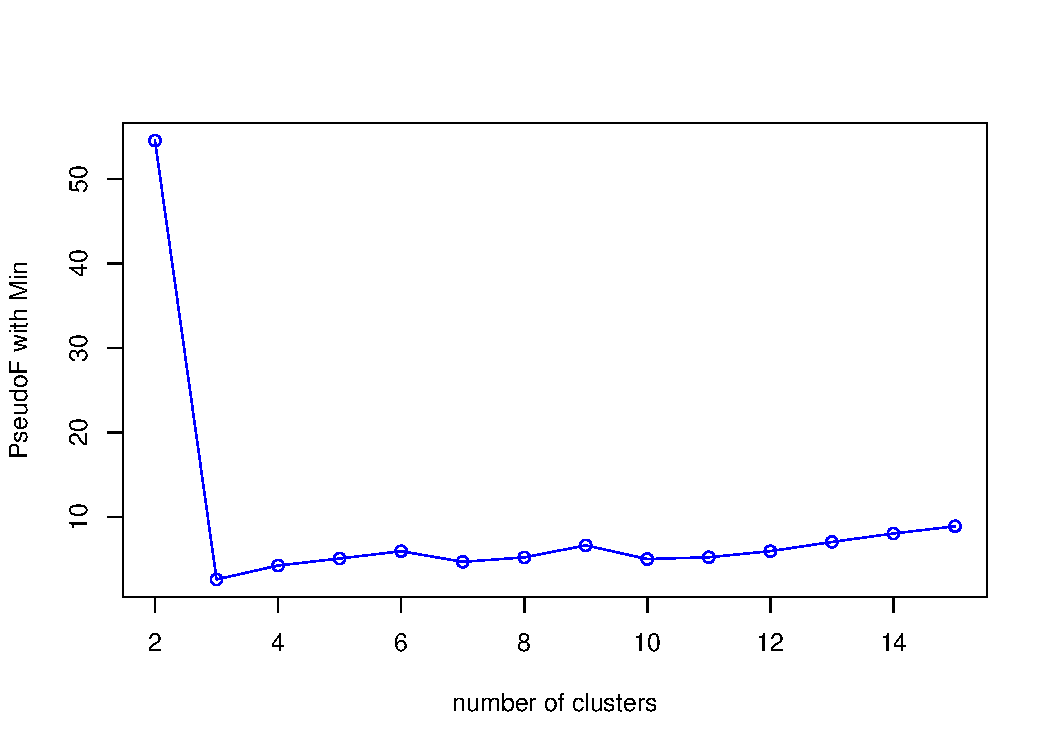
\includegraphics[width=0.4\hsize]{norm-PseudoFwithMin}
}~
\subfigure[変動値]{
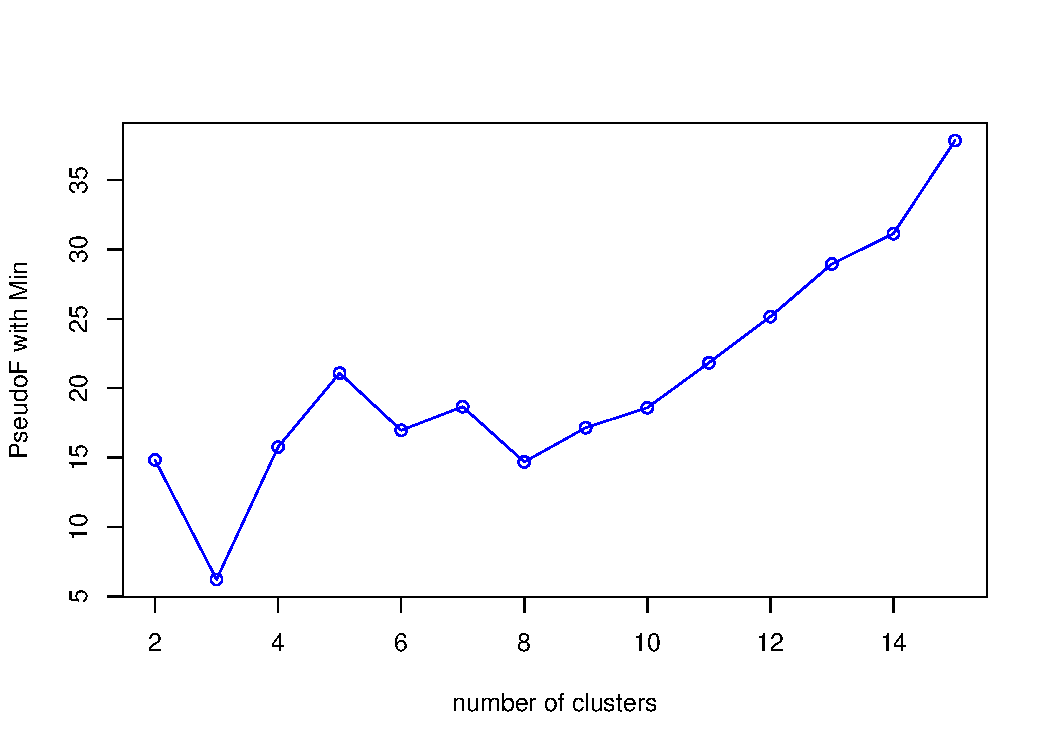
\includegraphics[width=0.4\hsize]{diff-PseudoFwithMin}
}
\caption{クラスタ数と Pseudo F with Min の関係}
\label{PseudoFwithMinPlot}
\end{center}
\end{figure}
図より,実測値の場合にはクラスタ数 2 で,変動値の場合にはクラスタ数 15 でそれぞれ Pseudo F with Min が最大になることがわかる.

まずは,実測値を用いたクラスタリングを行った.横軸に示すそれぞれのクラスタについて,各時間帯の区間データ数を図 (a)に,各曜日の区間データ数をそれぞれ図 (b) に積み上げグラフで示している.
\begin{figure}[tb]
\begin{center}
\subfigure[時間帯での分類]{
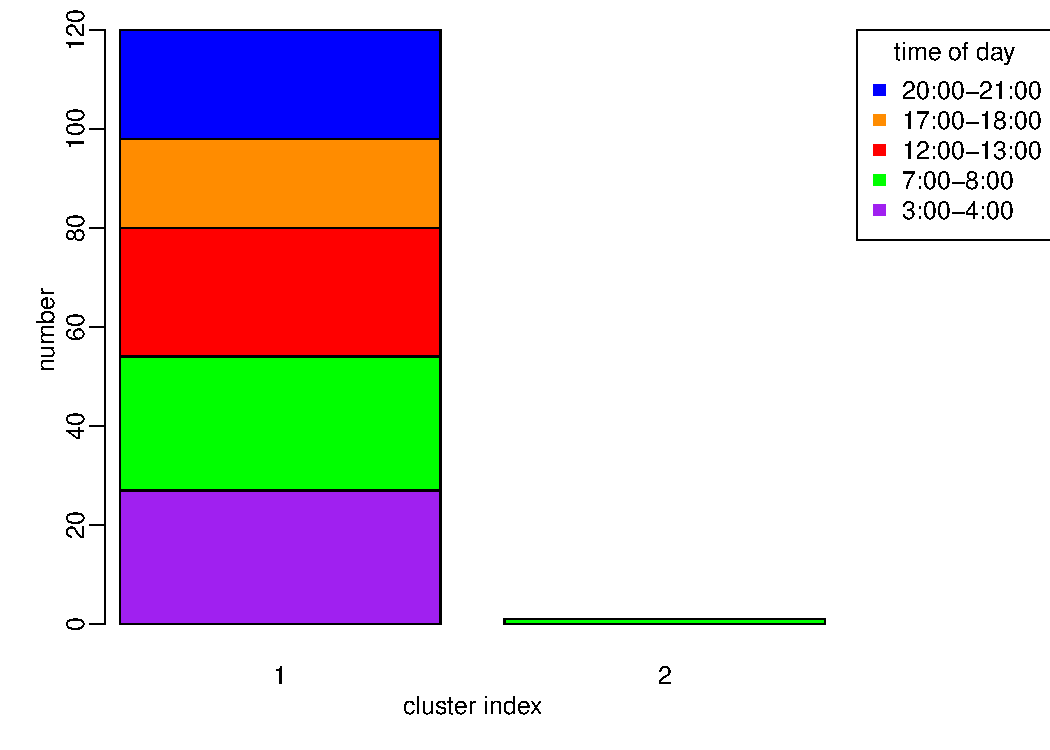
\includegraphics[width=0.4\hsize]{num-norm-eucl-ward-2-timezone.pdf}
}~
\subfigure[曜日での分類]{
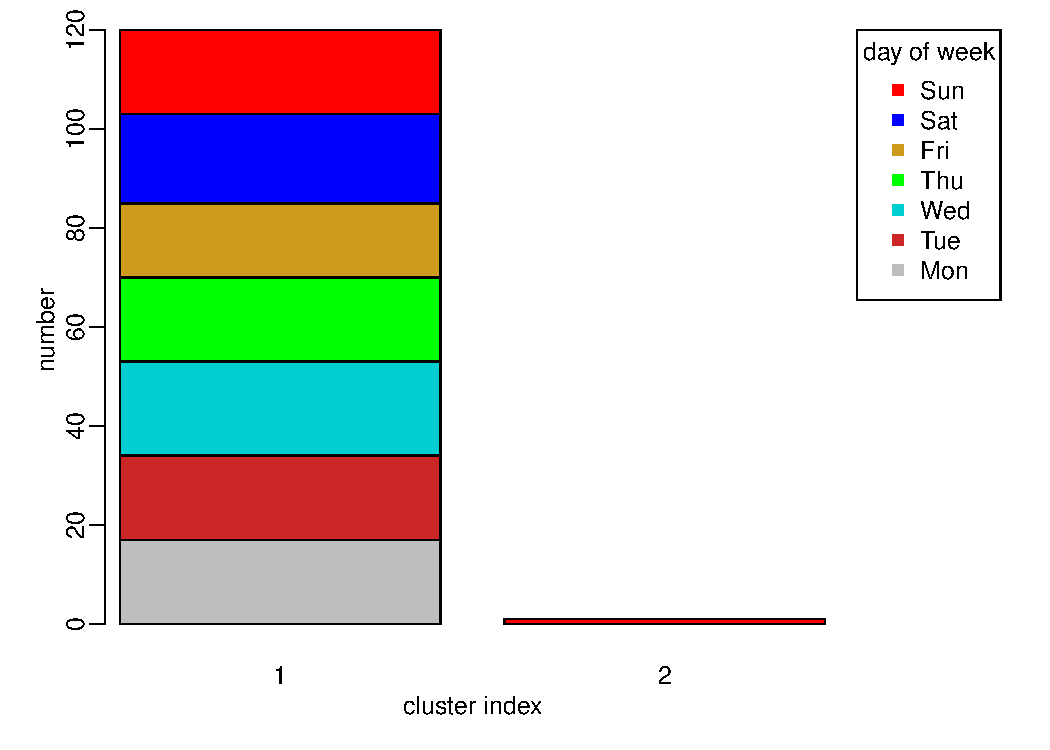
\includegraphics[width=0.4\hsize]{num-norm-eucl-ward-2-day.pdf}
}\\
\caption{実測値のクラスタリング結果}
\label{norm}
\end{center}
\end{figure}
図より,ただ一つの区間データを除いた区間データがクラスタ 1 に分類されていることがわかる.この結果からは曜日や時間帯による傾向を見出すことはできない.また,この区間データは 3/15(日)7:00-8:00 に得られる計測データであった.この区間データがどのようなものであったのかを調べるため比較対象として同曜日,時間帯の3/8(日)7:00-8:00 を用い,応答遅延の実測値の回帰結果を図 3 に,モデルパラメータを表 1 に示す.
図 3 の赤線は回帰線,青線は応答遅延の実測値,緑線は信頼区間 95\% を表す.
\begin{figure}[tb]
\begin{center}
\subfigure[3/8(日)7:00-8:00]{
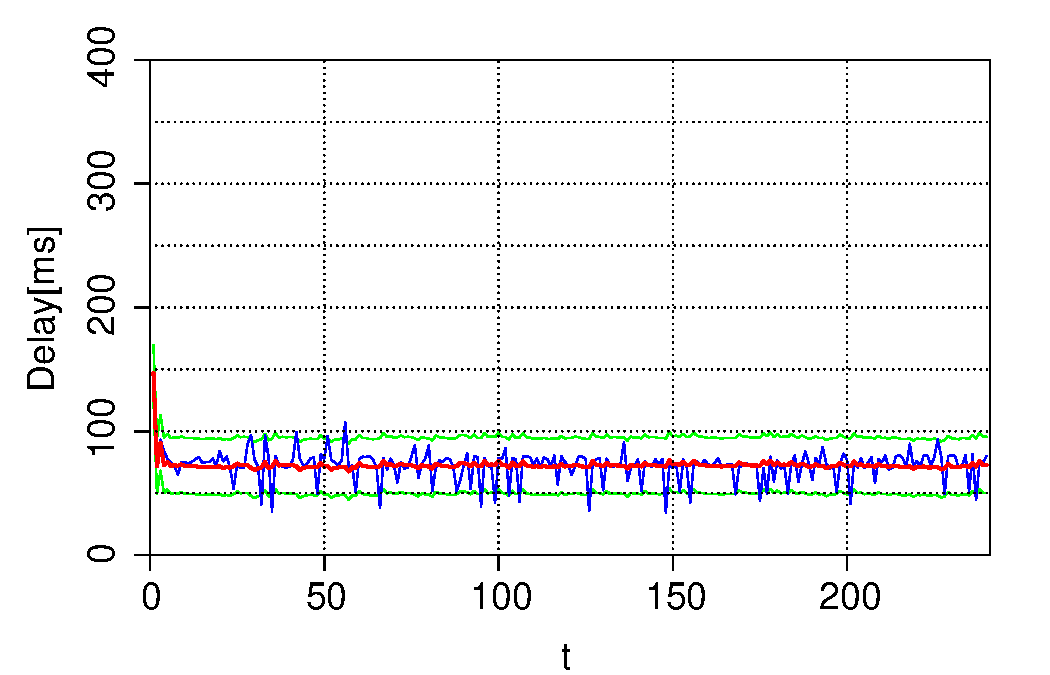
\includegraphics[width=0.4\hsize]{0308_07-plot.pdf}
}~
\subfigure[3/15(日)7:00-8:00]{
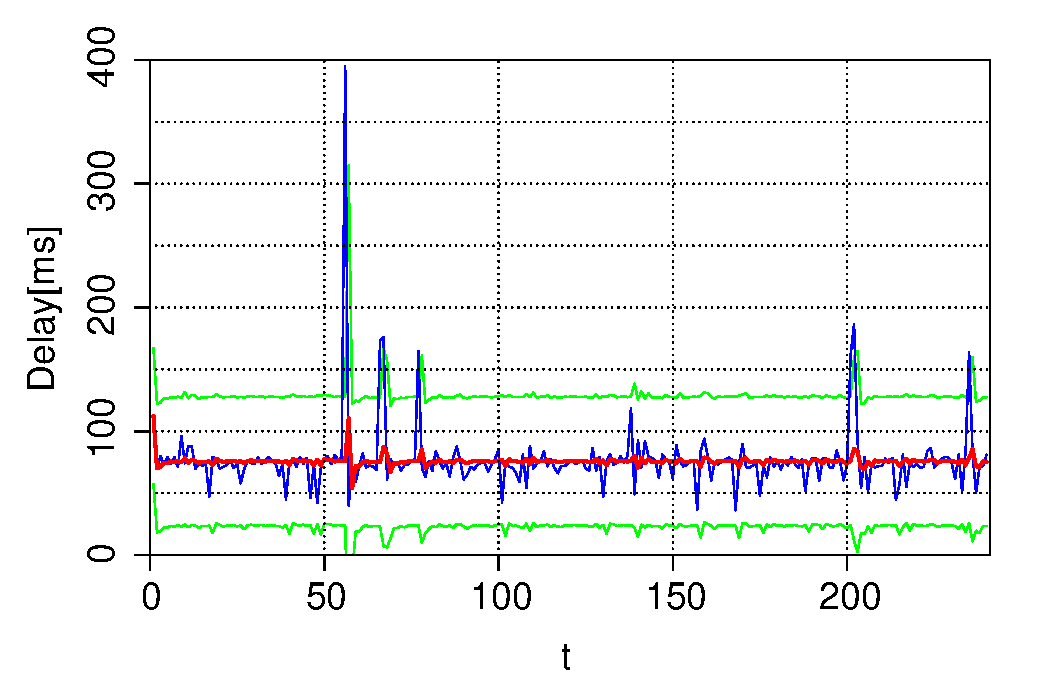
\includegraphics[width=0.4\hsize]{0315_07-plot.pdf}
}
\caption{応答遅延の実測値の回帰結果}
\end{center}
\end{figure}
\begin{table}[tb]
\centering
\caption{応答遅延の実測値のモデルパラメータ}
\begin{tabular}{|c|c|c|}
\hline
& 3/8(日)7:00-8:00& 3/15(日)7:00-8:00\\
\hline
$a_1$&51.12567&37.37011\\
\hline
$a_2$&0.04495093&0.5457383\\
\hline
$b_1$&0.2469837&-0.03917198\\
\hline
$b_2$&-0.1671403&-0.4350504\\
\hline
$c$&-0.264098&-0.06346395\\
\hline
$\omega$&7.901796&703.1791\\
\hline
$\alpha_1$&1e-08&0.09949149\\
\hline
$\beta_1$&0.9412245&1e-08\\
\hline
\end{tabular}
\end{table}
図3 より,3/15(日)7:00-8:00 の実測値の特徴としては 400 ms 程のかなり大きな応答遅延が発生していることがわかる. 400 ms は平時に単発的に発生する大きな応答遅延の中でも比較的大きな値である.さらに,100 ms 以上の大きな応答遅延も一時間のうちに 5 回発生しており,この発生回数も多いような印象を受ける.

これらの特徴が他の区間データとの大きなモデルパラメータの違いを生じさせ,このデータのみが異なるクラスタに属するという結果につながったのではないかと考えられる.特に表 1 より,ARMA-GARCH モデルにおけるノイズ項が従う分散に対する定数項のパラメータ $\omega$ に大きな差を生じさせたのではないかと思われる.

次に,変動値に対するクラスタリング結果を図 4 に示す.
\begin{figure}[tb]
\begin{center}
\subfigure[時間帯での分類]{
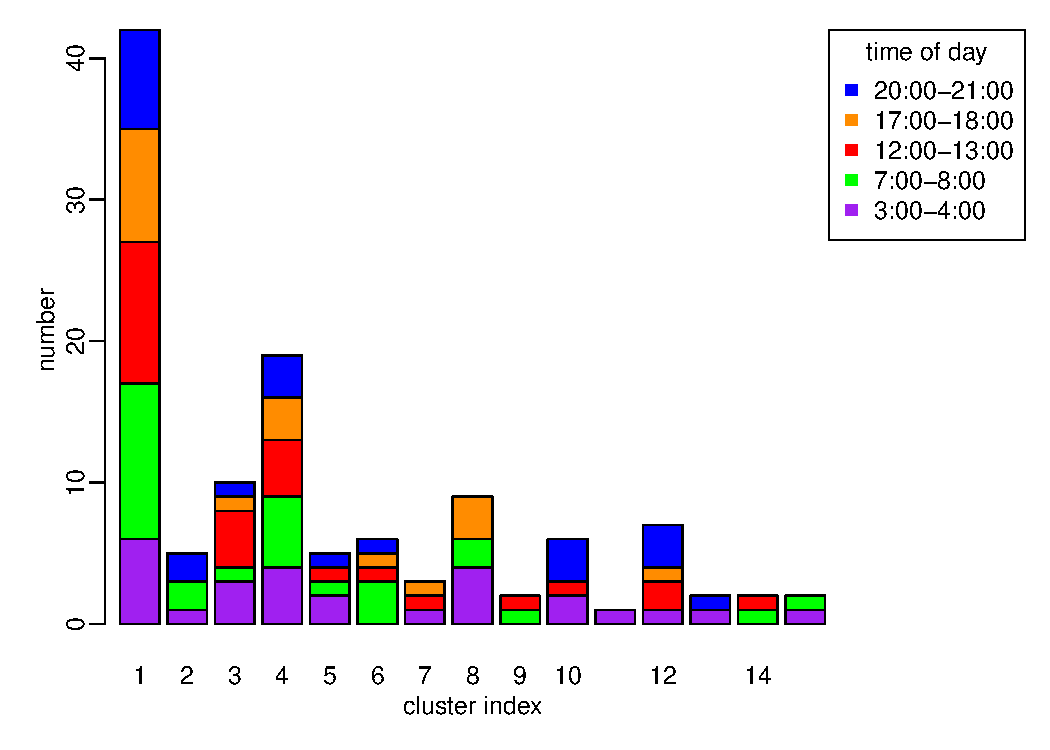
\includegraphics[width=0.4\hsize]{num-diff-eucl-ward-15-timezone.pdf}
}~
\subfigure[曜日での分類]{
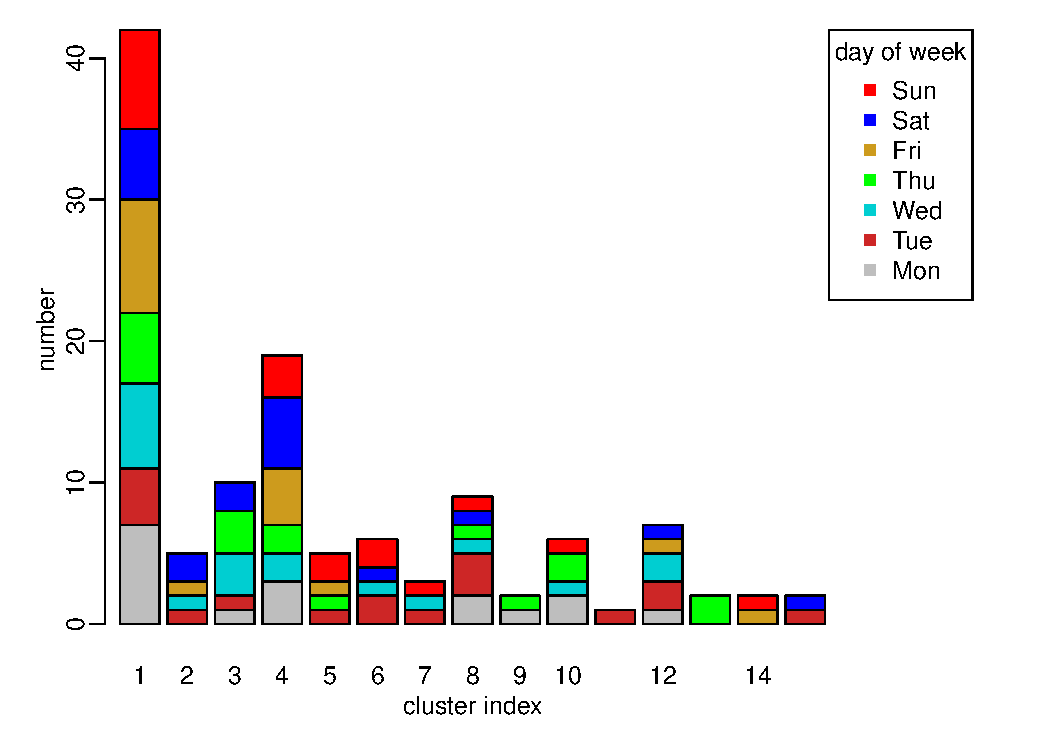
\includegraphics[width=0.4\hsize]{num-diff-eucl-ward-15-day.pdf}
}\\
\caption{変動値のクラスタリング結果}
\label{norm}
\end{center}
\end{figure}
図 4 より,クラスタリング結果に曜日や時間帯による偏りはあることが見て取れる.しかしながら,クラスタの要素数が 10 以下の小さなクラスタがほとんどで,かつ 15 個もあるクラスタに区間データが散らばっており,それらの間に共通する傾向を見出すことが困難であった.

以上の結果より,前処理を行わないクラスタリングパラメータを用いてクラスタリングを行っても,曜日や時間帯に依存した傾向を見出せるような結果を得ることは困難であることが分かった.したがって,IN 原稿のような,モデルパラメータの各分布を揃えるための標準化や,クラスタの過度な細分化を防ぐための主成分分析は有効な処理であったと思われる.
\end{document}